
\documentclass[tikz,convert={convertexe={magick.exe}}]{standalone}
%\documentclass[tikz,convert]{standalone}
\usetikzlibrary{arrows}

\usepackage{ifthen}

\usepackage{amssymb}
\newcommand{\into}{\mathop{\lrcorner}}

\usetikzlibrary{snakes}
\usetikzlibrary{decorations.pathmorphing}

\begin{document}
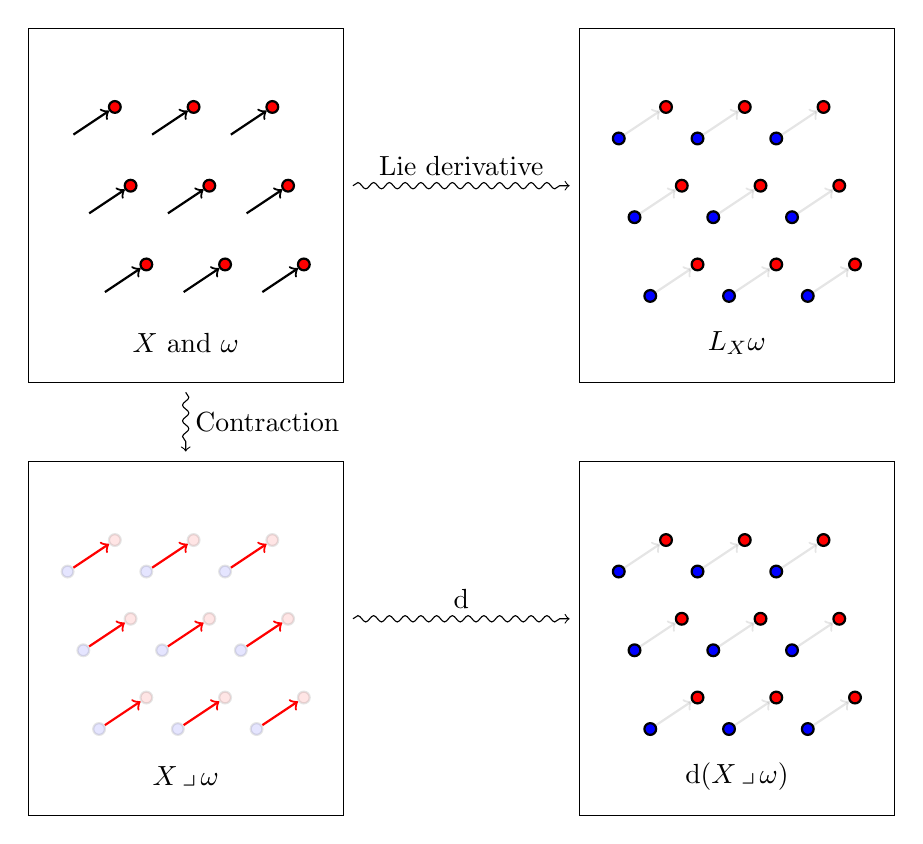
\begin{tikzpicture}

\tikzstyle atom=[circle, draw, inner sep=1.2pt, fill=red, thick]
\tikzstyle bigatom=[circle, draw, inner sep=1.5pt, fill=red, thick]
\tikzstyle snakearrow=[->,decorate,decoration={snake,amplitude=.4mm,segment length=2mm,post length=1mm}]

\begin{scope}

\draw (-2,-2.5) rectangle (2,2);
\node at (0,-2) {$X$ and $\omega$};

\foreach \x in {-1,...,1}
\foreach \y in {-1,...,1} {
\node[bigatom] (A\x\y) at (\x-.2*\y+.3,\y) {};
\node[bigatom,fill=blue,opacity=0] (B\x\y) at (\x-.2*\y-.3,\y-.4) {};
\draw[->,thick] (B\x\y)--(A\x\y);
}

\node (XS) at (0,-2.5) {};
\node (XE) at (2,0) {};
\end{scope}

\begin{scope}[xshift=7cm]

\draw (-2,-2.5) rectangle (2,2);
\node at (0,-2) {$L_X \omega$};

\foreach \x in {-1,...,1}
\foreach \y in {-1,...,1} {
\node[bigatom] (A\x\y) at (\x-.2*\y+.3,\y) {};
\node[bigatom,fill=blue] (B\x\y) at (\x-.2*\y-.3,\y-.4) {};
\draw[->,thick,opacity=0.1] (B\x\y)--(A\x\y);
}

\node (YW) at (-2,0) {};
\end{scope}

\begin{scope}[yshift=-5.5cm]

\draw (-2,-2.5) rectangle (2,2);
\node at (0,-2) {$X \into \omega$};

\foreach \x in {-1,...,1}
\foreach \y in {-1,...,1} {
\node[bigatom,opacity=0.1] (A\x\y) at (\x-.2*\y+.3,\y) {};
\node[bigatom,fill=blue,opacity=0.1] (B\x\y) at (\x-.2*\y-.3,\y-.4) {};
\draw[->,thick,red] (B\x\y)--(A\x\y);
}

\node (ZN) at (0,2) {};
\node (ZE) at (2,0) {};
\end{scope}

\begin{scope}[xshift=7cm,yshift=-5.5cm]

\draw (-2,-2.5) rectangle (2,2);
\node at (0,-2) {$\mathrm{d}(X \into \omega)$};

\foreach \x in {-1,...,1}
\foreach \y in {-1,...,1} {
\node[bigatom] (A\x\y) at (\x-.2*\y+.3,\y) {};
\node[bigatom,fill=blue] (B\x\y) at (\x-.2*\y-.3,\y-.4) {};
\draw[->,thick,opacity=0.1] (B\x\y)--(A\x\y);
}

\node (WW) at (-2,0) {};
\end{scope}

\draw[snakearrow] (XE) -- (YW) node[midway, above] {Lie derivative};
\draw[snakearrow] (ZE) -- (WW) node[midway, above] {$\mathrm{d}$};
\draw[snakearrow] (XS) -- (ZN) node[midway, right] {Contraction};

\end{tikzpicture}
\end{document}